\chapter{THỰC NGHIỆM VÀ ĐÁNH GIÁ KẾT QUẢ NGHIÊN CỨU}
\label{Chapter4}

\section{Quy trình thực nghiệm}
Toàn bộ quy trình triển khai và đánh giá thực nghiệm tất cả các khâu trong khung phương pháp (framework) đều được lập trình bằng ngôn ngữ Python, kết hợp cùng framework học sâu PyTorch và thư viện mã nguồn mở Transformers (Hugging Face).

Về môi trường phần cứng, quá trình huấn luyện và kiểm thử các mô hình (\textbf{mBERT}, \textbf{PhoBERT} và \textbf{mModernBERT}) được thực hiện trên hệ thống máy chủ hiệu năng cao. Hệ thống này được trang bị vi xử lý CPU Intel Xeon® E5-2686 v4 (72 cores), dung lượng bộ nhớ trong (RAM) lên đến 258 GB, cùng bộ xử lý đồ họa (GPU) NVIDIA GeForce RTX 3090 sở hữu 24GB VRAM (năng lực tính toán đạt 35.3 TFLOPS), đảm bảo khả năng xử lý song song khối lượng dữ liệu lớn.

Đối với khâu chuẩn bị dữ liệu, tập ngữ liệu sau khi trải qua quá trình gán nhãn và giảm mẫu đa số (Undersampling) được phân chia ngẫu nhiên thành ba tập con độc lập: tập huấn luyện (Training set), tập kiểm định (Validation set) và tập kiểm thử (Test set) với tỷ lệ phân bổ tương ứng là 90:5:5.

Về quá trình huấn luyện, cấu hình của ba mô hình được thiết lập chi tiết dựa trên các siêu tham số trình bày tại Bảng \ref{tab:hyperparameters_detail}. Nhằm tối ưu hóa thời gian tính toán và ngăn chặn hiện tượng quá khớp (overfitting), kỹ thuật dừng sớm (Early Stopping) được tích hợp vào quy trình. Cụ thể, tiến trình huấn luyện sẽ tự động chấm dứt nếu độ đo hiệu năng trên tập kiểm định không ghi nhận sự cải thiện nào sau hai chu kỳ (epochs) liên tiếp.

\begin{table}[H]
    \centering
    \renewcommand{\arraystretch}{1.5} 
    \caption{Cấu hình siêu tham số chi tiết cho từng mô hình thực nghiệm.}
    \label{tab:hyperparameters_detail}
    \begin{tabular}{|p{5.5cm}|c|c|c|}
        \hline
        \textbf{Siêu tham số} & \textbf{mBERT} & \textbf{PhoBERT} & \textbf{mModernBERT} \\
        \hline
        Số lượng nhãn phân loại (\textit{n\_classes}) & 28 & 28 & 28 \\
        \hline
        Độ dài chuỗi tối đa (\textit{max\_len}) & 512 & \textbf{256} & 512 \\
        \hline
        Hệ số học (\textit{learning rate}) & $2.0 \times 10^{-5}$ & $2.0 \times 10^{-5}$ & $\mathbf{1.0 \times 10^{-5}}$ \\
        \hline
        Số vòng huấn luyện (\textit{epochs}) & 12 & 12 & 12 \\
        \hline
        Kích thước lô (\textit{batch\_size}) & 32 & 32 & 32 \\
        \hline
        Tích lũy gradient (\textit{accumulate\_steps}) & 2 & 2 & 2 \\
        \hline
        Kích thước lô hiệu dụng (\textit{effective batch}) & 64 & 64 & 64 \\
        \hline
        Tỷ lệ Dropout & 0.1 & 0.1 & 0.1 \\
        \hline
        Độ chính xác hỗn hợp (\textit{FP16}) & Có & Có & Có \\
        \hline
        Tham số $\beta$ (CB-Loss) & 0.999 & 0.999 & 0.999 \\
        \hline
        Số lượng khoảng (\textit{GHM bins}) & 10 & 10 & 10 \\
        \hline
    \end{tabular}
\end{table}

\section{Kết quả thực nghiệm}

\subsection{Kết quả quá trình thu thập, xây dựng, tiền xử lý và gán nhãn dữ liệu}
Thông qua các biểu đồ phân phối tập dữ liệu sau quá trình thu thập và xây dựng, tiền xử lý (Hình \ref{fig:first_cbc} và Hình \ref{fig:first_vbc}) đều có thể thấy được tập ngữ liệu mang đặc tính mất cân bằng sâu sắc mang tính tự nhiên (Long-tail distribution). Các chủ đề mang tính thời sự hoặc giải trí cao (như \texttt{news}, \texttt{music}) thu hút lượng tương tác áp đảo, trong khi các danh mục khác lại vô cùng hạn chế. Sự phân bố không cân bằng này chính là minh chứng cho thấy nếu sử dụng phương pháp luận truyền thống, mô hình sẽ hoàn toàn bị thiên kiến (bias) theo các chủ đề phổ biến. Do đó, việc framework tích hợp \textbf{cơ chế gán nhãn bán tự động} (kết hợp luật từ vựng và sinh dữ liệu nhân tạo) cùng \textbf{hàm mất mát hỗn hợp (Mixture Loss)} là một bước đi mang tính chiến lược và bắt buộc.

\begin{figure}[H]
    \centering
    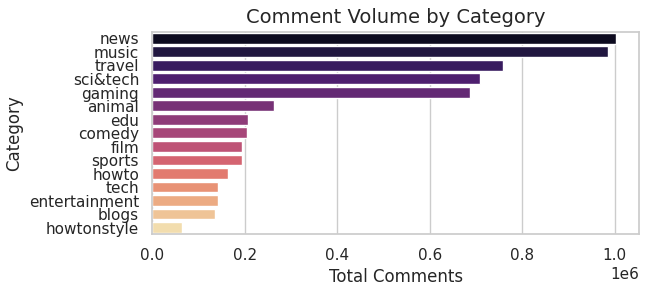
\includegraphics[width=0.8\textwidth]{Images/comment_by_cate.png}
    \caption{Phân phối dữ liệu số lượng bình luận sau quá trình thu thập và tiền xử lý theo các danh mục.}
    \label{fig:first_cbc}
    \vspace{0.1cm}
\end{figure}

\begin{figure}[H]
    \centering
    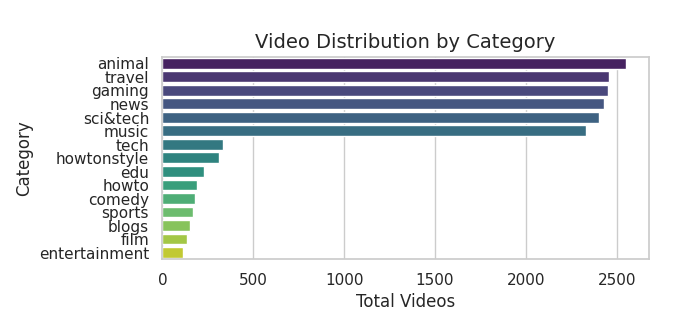
\includegraphics[width=0.8\textwidth]{Images/vid_by_cate.png}
    \caption{Phân phối dữ liệu số lượng video sau quá trình thu thập và tiền xử lý theo các danh mục.}
    \label{fig:first_vbc}
    \vspace{0.1cm}
\end{figure}

Biểu đồ violin (Hình \ref{fig:first_cmt_violin}) chỉ ra rằng tuyệt đại đa số bình luận của người dùng mạng xã hội Việt Nam thường có độ dài vô cùng ngắn (tập trung ở ngưỡng dưới 20 từ, kể cả icons). Việc phân loại cảm xúc vi mô (fine-grained emotions) trên các đoạn văn bản thiếu hụt ngữ cảnh trầm trọng là một thách thức cực đại đối với học máy. Tuy nhiên, giới hạn này lại làm nổi bật tính đúng đắn trong việc lựa chọn và thiết kế framework. Nhờ việc tinh chỉnh các \textbf{kiến trúc Transformer tiên tiến (như mModernBERT với cơ chế Attention tối ưu)}, framework có đủ độ nhạy bén để trích xuất các dấu hiệu ngữ nghĩa tinh tế nhất chỉ từ một vài từ khóa, vượt qua rào cản về độ dài văn bản mà các mô hình biểu diễn ngữ nghĩa truyền thống thường thất bại.
Ngoài ra, sự xuất hiện của các điểm dị thường (outliers) kéo dài lên tới 250 tokens cho thấy độ nhiễu và tính đa dạng hóa của tập ngữ liệu.

\begin{figure}[H]
    \centering
    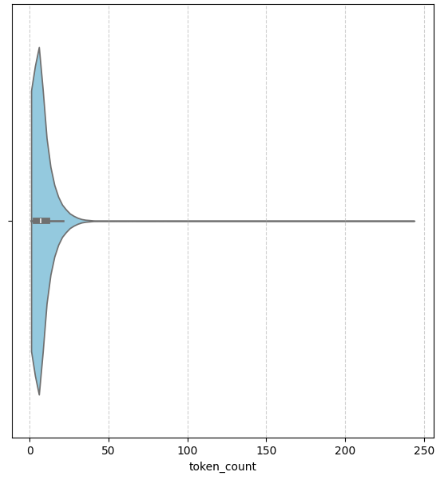
\includegraphics[width=0.8\textwidth]{Images/stats_tk.png}
    \caption{Biểu đồ violin phân phối số lượng từ trong từng bình luận.}
    \label{fig:first_cmt_violin}
    \vspace{0.1cm}
\end{figure}

Kết quả của quá trình gán nhãn bán tự động được thể hiện qua phân phối dữ liệu dựa theo các nhóm cảm xúc (Hình \ref{fig:label_anno_dist}) bộc lộ rõ rệt cấu trúc phân phối đuôi dài (long-tail distribution) mang tính tự nhiên. Các nhãn thuộc nhóm tích cực áp đảo hoàn toàn các nhãn thuộc nhóm tiêu cực. Đồng thời, việc số lượng nhãn trung tính (neutral) đột biến lại là một tín hiệu tốt và mang tính bảo chứng. Vì thực tế trên mạng xã hội (YouTube, TikTok, Facebook), 70\% - 80\% bình luận thực tế là vô thưởng vô phạt, ngắn gọn, hoặc thuần túy trần thuật (ví dụ: "video hay", "chấm", "đã xem", "ông A đi xe màu đỏ").

Đồng thời, bức tranh phân bố cảm xúc cũng cho thấy sự tương đồng với tập dữ liệu GoEmotions đã được kiểm chứng nghiêm ngặt (như Hình \ref{fig:label_goemo_dist}). Sự nhất quán về mặt phân phối này khẳng định rằng sự kết hợp giữa luật từ vựng (rule-based) và mô hình ngôn ngữ (Encoder) trong khung phương pháp đã thành công trong việc chuyển giao tri thức (knowledge transfer) từ chuyên gia con người sang hệ thống máy tính với độ sai số được kiểm soát chặt chẽ.

\begin{figure}[H]
    \centering
    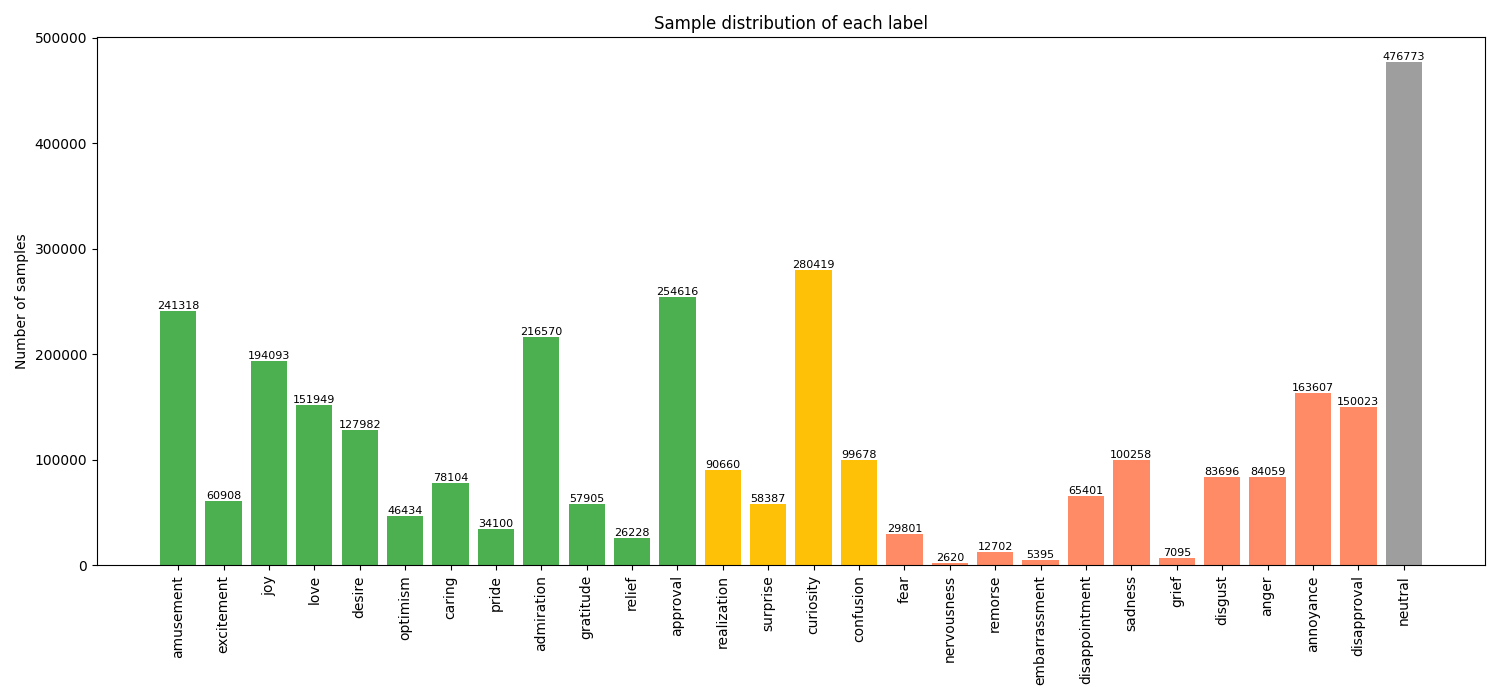
\includegraphics[width=0.8\textwidth]{Images/label_distribution.png}
    \caption{Biểu đồ phân phối dữ liệu theo các nhóm cảm xúc (xanh - tích cực, đỏ - tiêu cực, vàng - nhập nhằng, xám - trung tính) sau khi được gán nhãn.}
    \label{fig:label_anno_dist}
    \vspace{0.1cm}
\end{figure}

\begin{figure}[H]
    \centering
    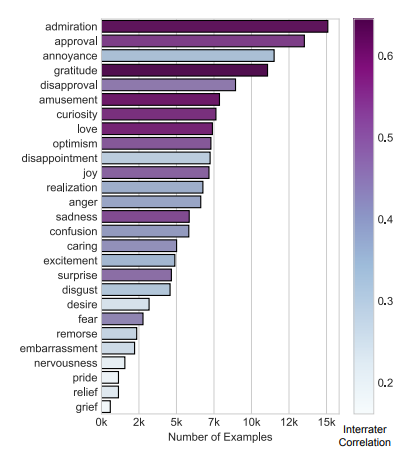
\includegraphics[width=0.8\textwidth]{Images/goemo_labeldist.png}
    \caption{Biểu đồ phân phối dữ liệu theo các cảm xúc vi mô trong tập GoEmotions.}
    \label{fig:label_goemo_dist}
    \vspace{0.1cm}
    {\small Nguồn: \parencite{demszky2020goemotions}}
\end{figure}

\subsection{Kết quả quá trình huấn luyện mô hình}
\begin{figure}[H]
    \centering
    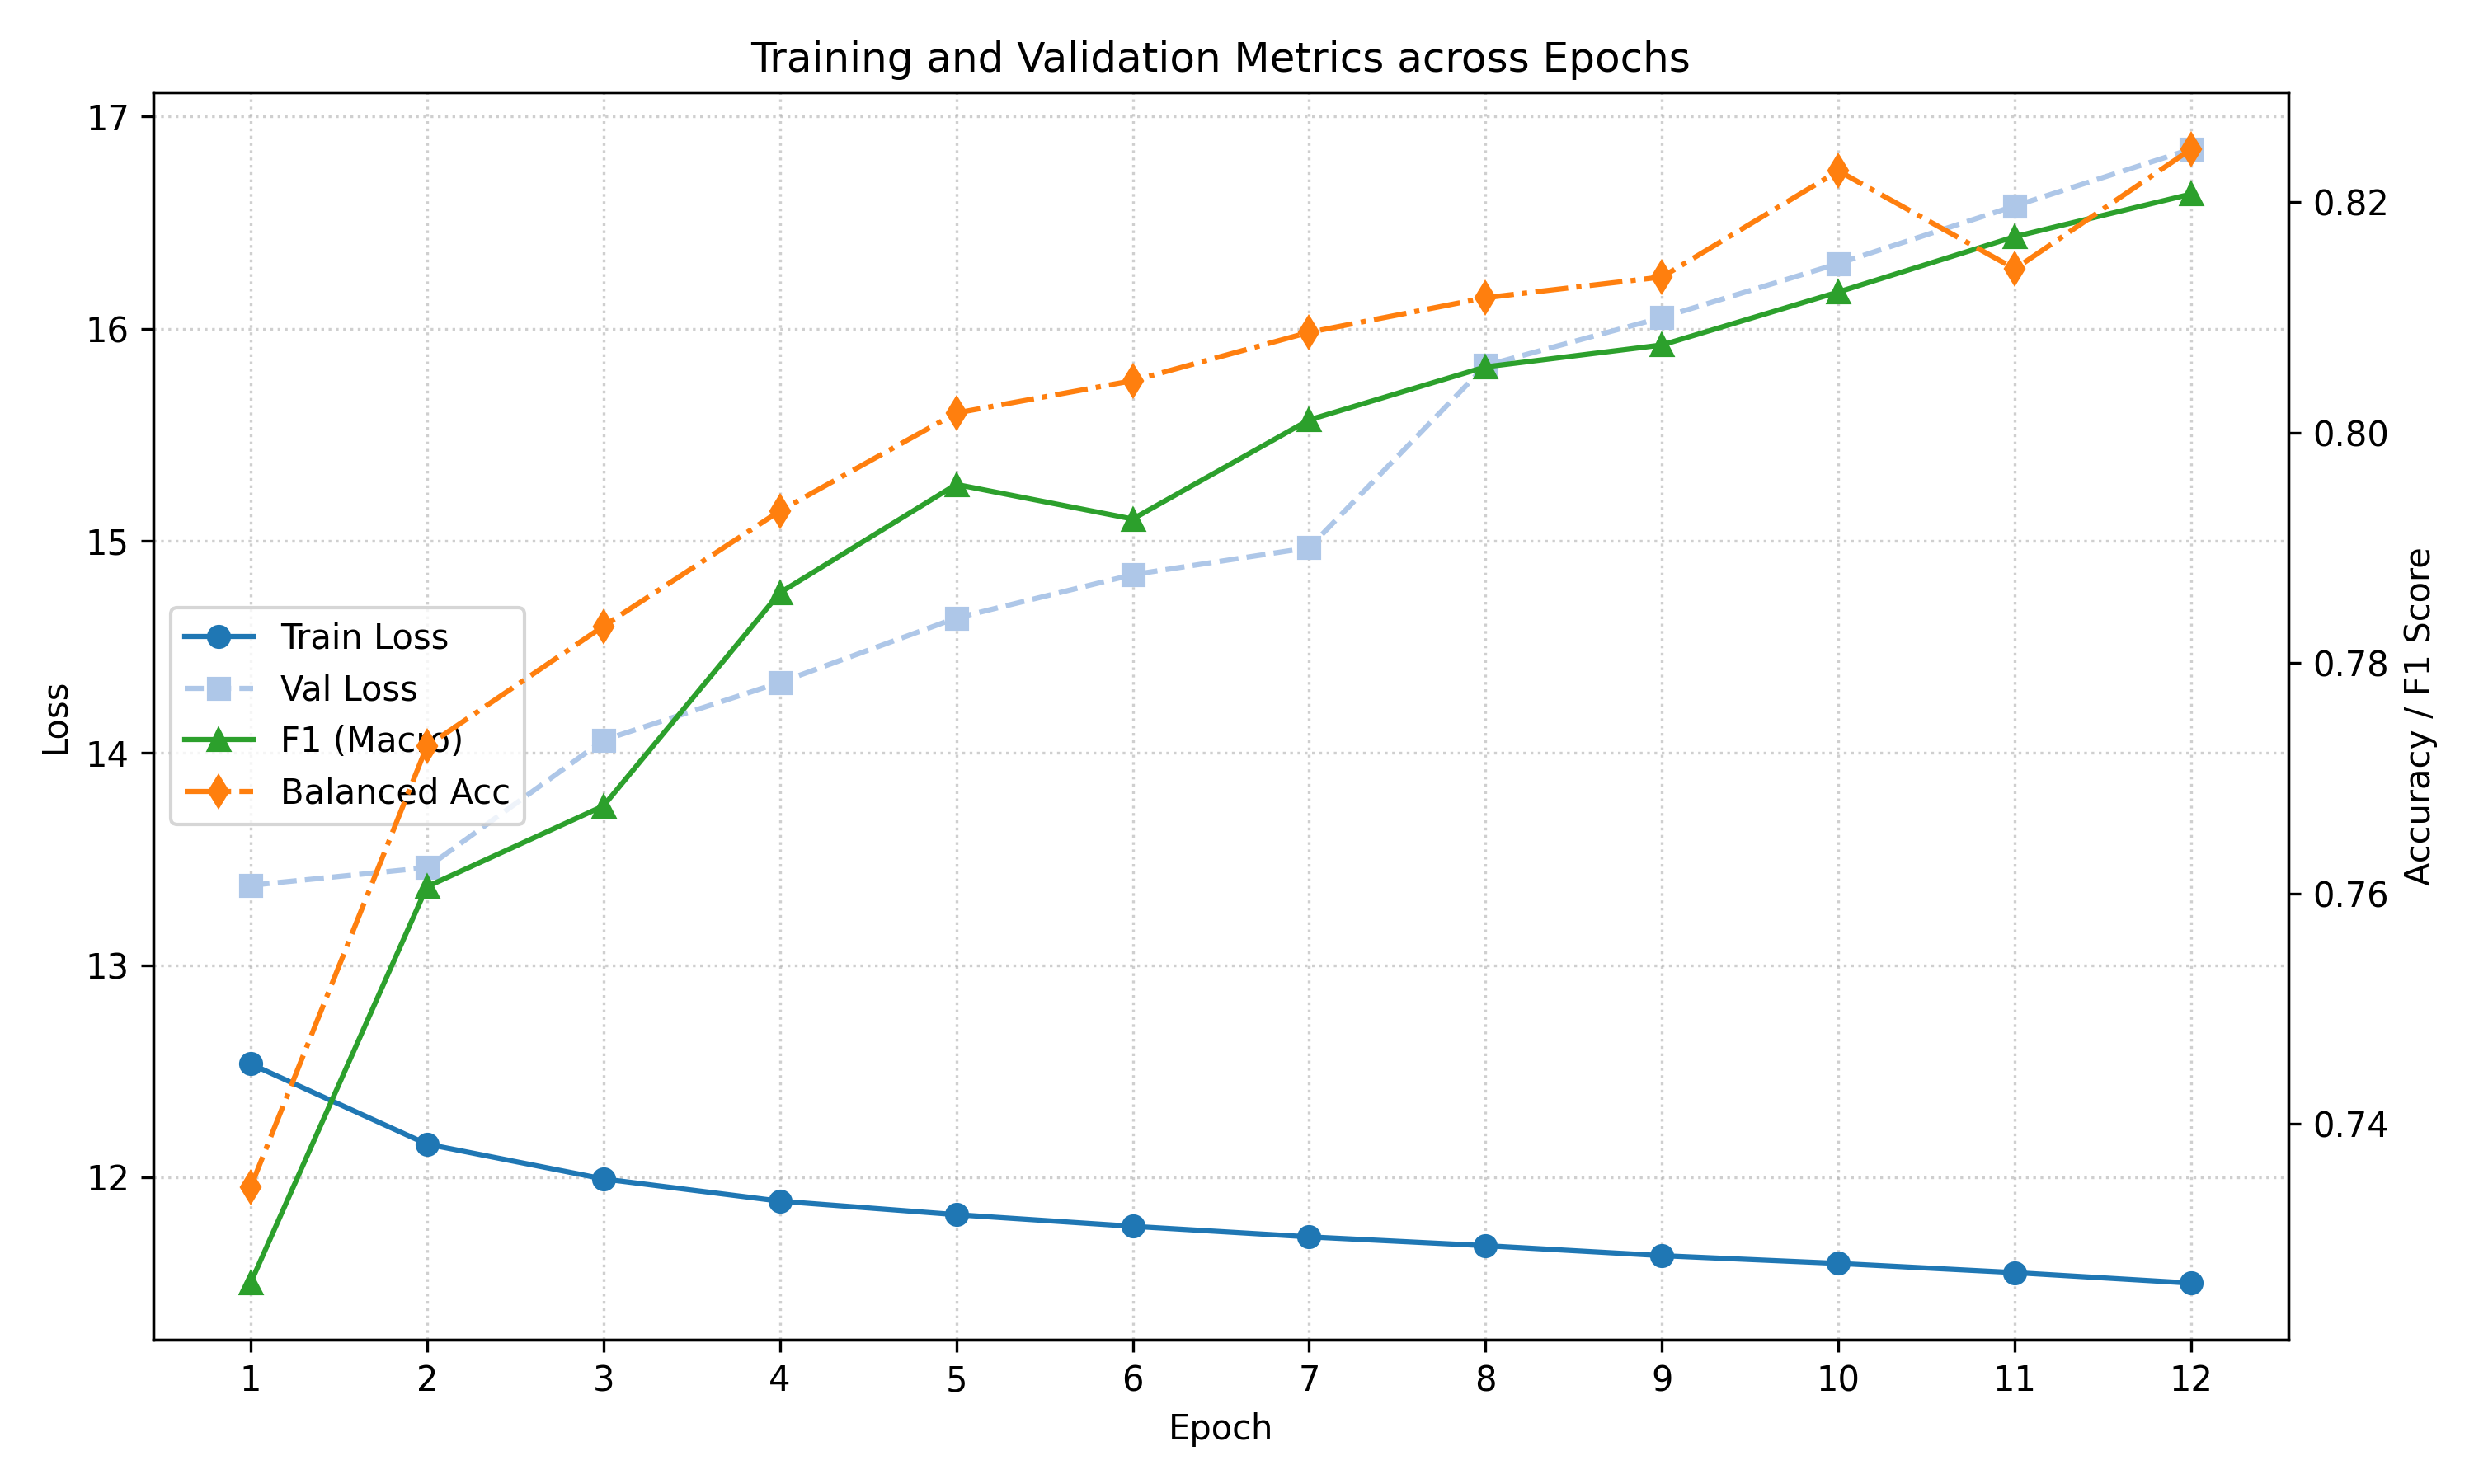
\includegraphics[width=0.8\textwidth]{Images/eps_mbert.png}
    \caption{Biểu đồ hành vi trong quá trình hiệu chỉnh mô hình mBERT.}
    \label{fig:eps_mbert}
    \vspace{0.1cm}
\end{figure}

\begin{figure}[H]
    \centering
    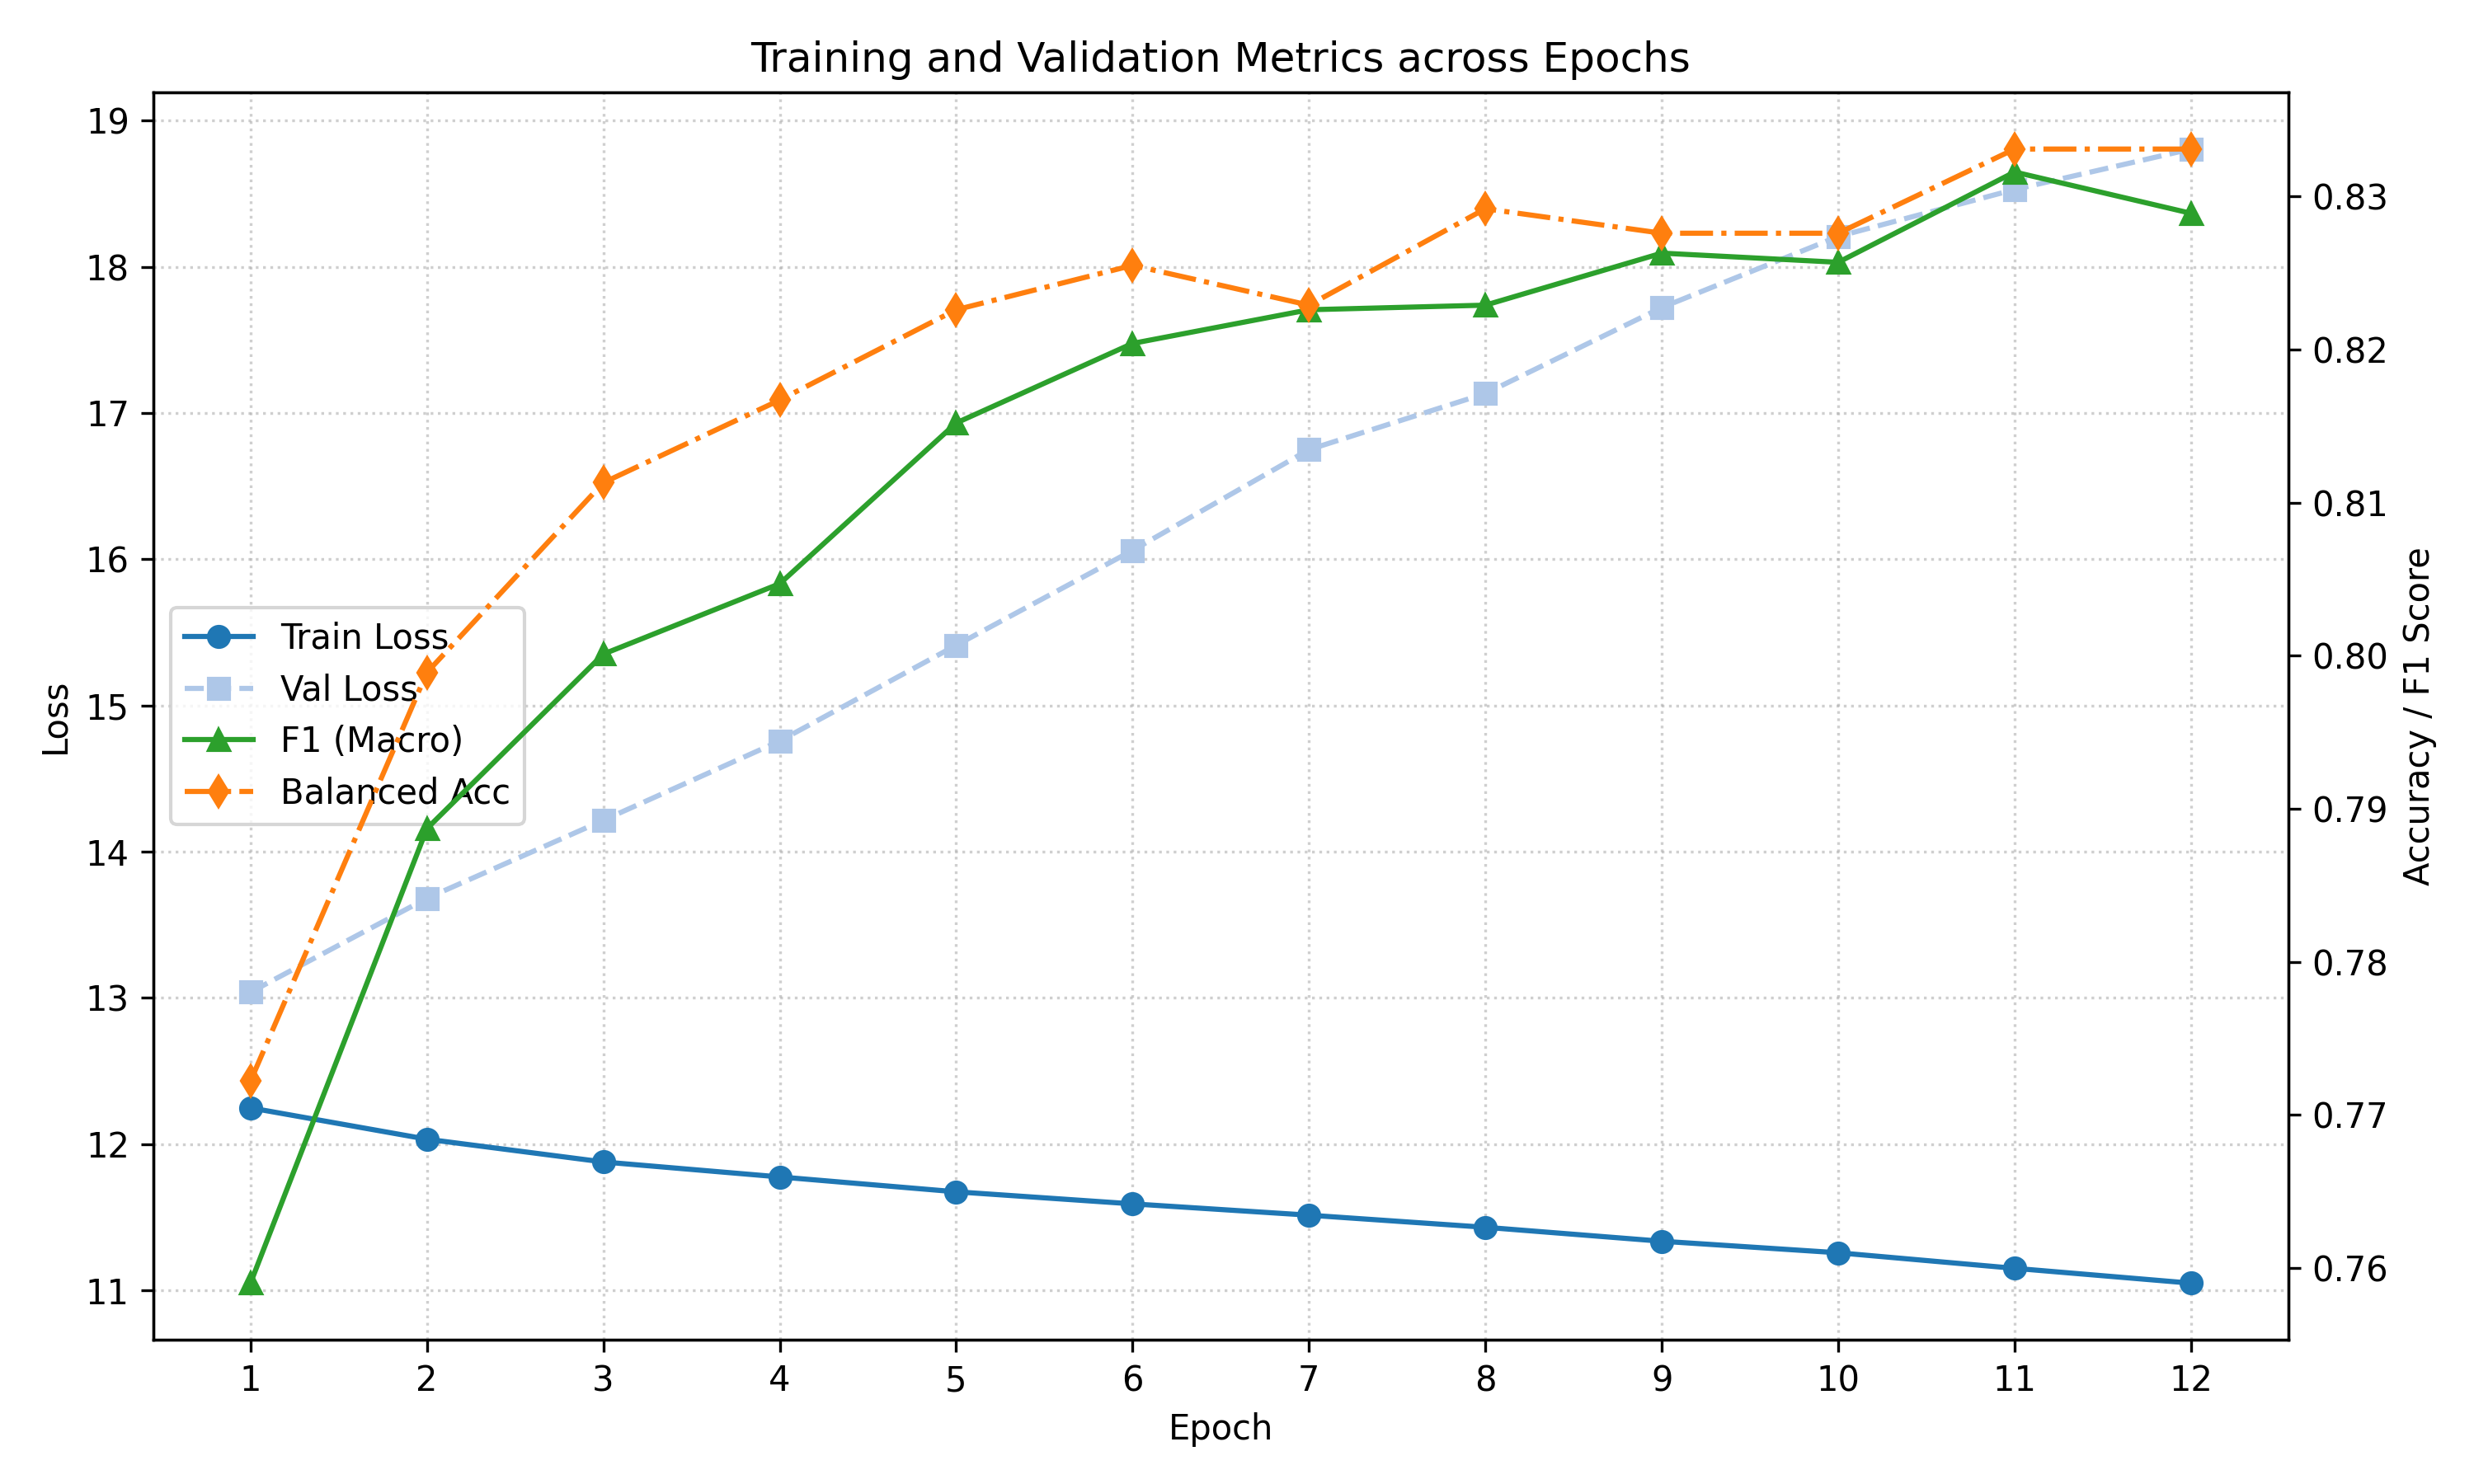
\includegraphics[width=0.8\textwidth]{Images/eps_phobert.png}
    \caption{Quá trình hiệu chỉnh mô hình phoBERT.}
    \label{fig:eps_phobert}
    \vspace{0.1cm}
\end{figure}

\begin{figure}[H]
    \centering
    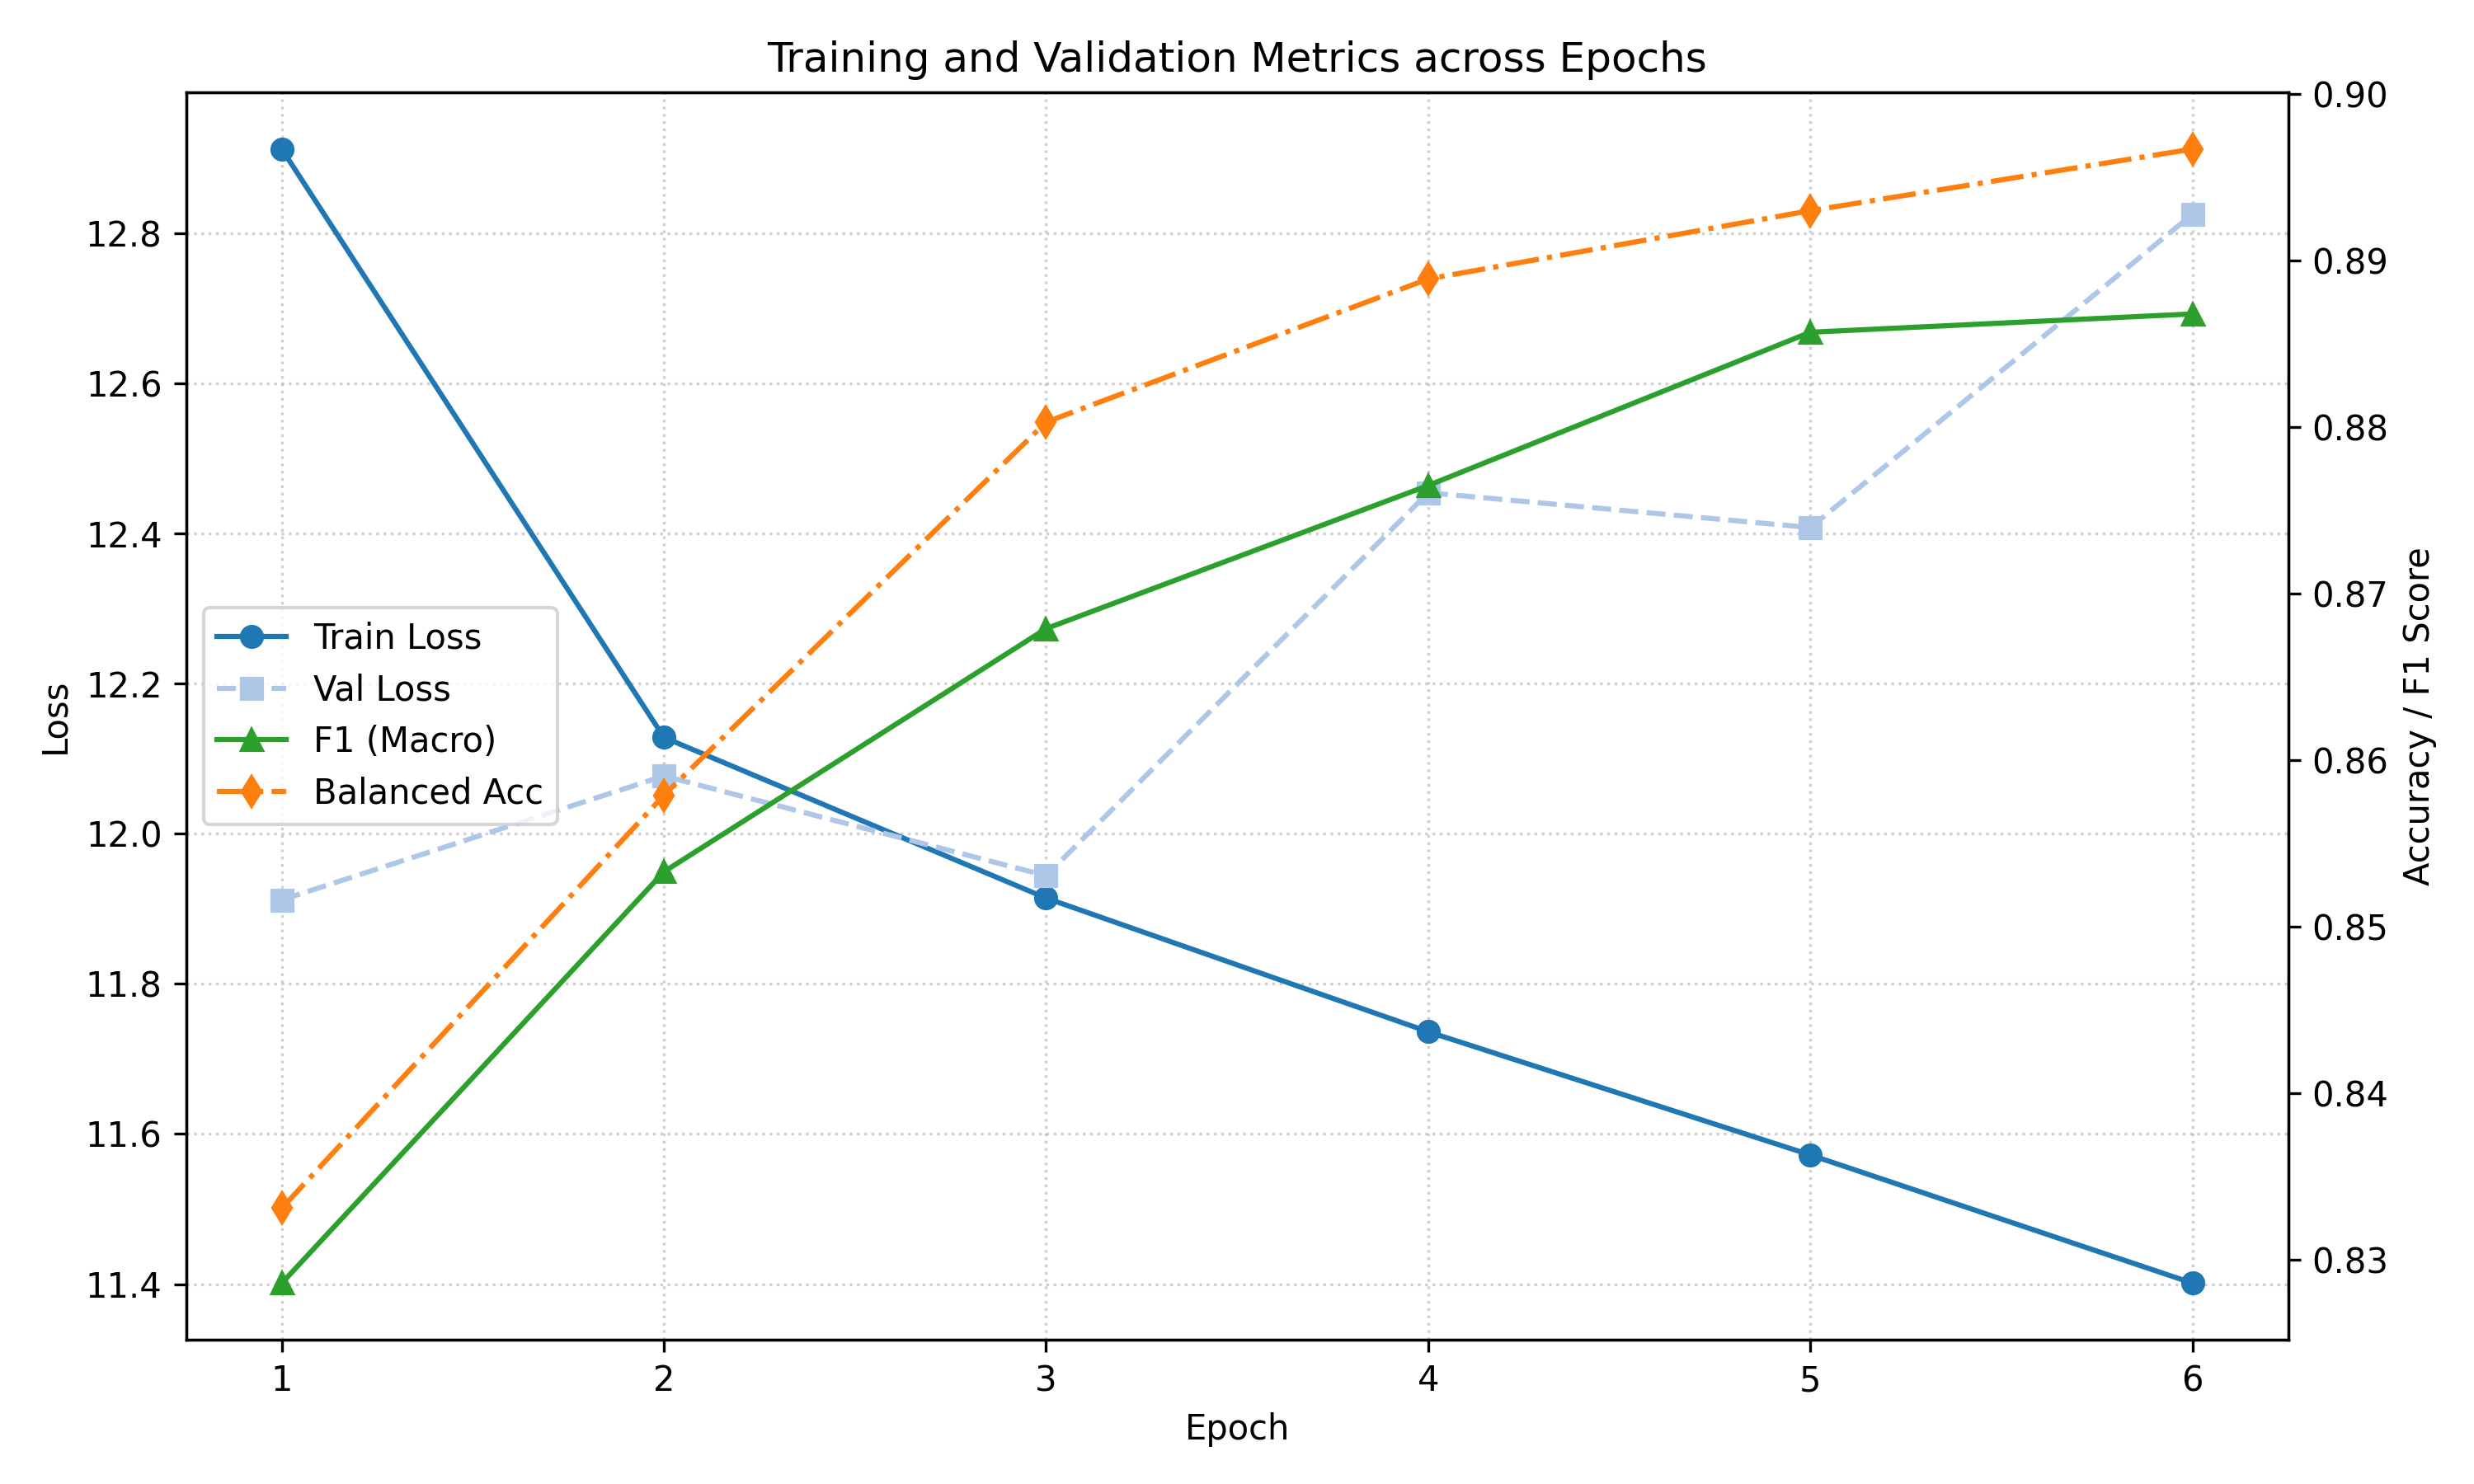
\includegraphics[width=0.8\textwidth]{Images/eps_mmbert.png}
    \caption{Quá trình hiệu chỉnh mô hình mModernBERT.}
    \label{fig:eps_modernbert}
    \vspace{0.1cm}
\end{figure}

Từ ba biểu đồ quá trình huấn luyện trên tập dữ liệu lớn với gần 3 triệu điểm dữ liệu và trên 28 lớp không cân bằng (imbalance) (Hình \ref{fig:eps_mbert}, Hình \ref{fig:eps_phobert} và Hình \ref{fig:eps_modernbert}) cho thấy hiện tượng phân kỳ sớm của giá trị mất mát kiểm định. Tuy nhiên, nếu ta đi vào phân tích sâu hơn, thì có thể nhận thấy rằng đây hoàn toàn là đặc trưng toán học mong muốn khi kết hợp giữa CB-Loss và GHM Loss nhằm bảo vệ các lớp thiểu số.

Đồng thời, hiệu năng thực tế của mô hình (thể hiện qua F1-Macro và Balanced Accuracy) vẫn không hề suy giảm mà vẫn tăng trưởng ổn định. Đặc biệt, các kết quả cũng cho thấy rằng điểm dừng lý tưởng (Early Stopping) rơi vào khoảng 3-5 epoch đầu tiên.


\subsection{Kết quả quá trình kiểm thử mô hình}

\begin{table}[H]
    \centering
    \renewcommand{\arraystretch}{1.3} 
    \caption{Kết quả đánh giá hiệu năng tổng thể của các mô hình trên tập kiểm thử.}
    \label{tab:overall_results}
    \begin{tabular}{|l|c|c|c|}
        \hline
        \textbf{Mô hình} & \textbf{F1-Macro} & \textbf{Overall Accuracy} & \textbf{Balanced Accuracy} \\
        \hline
        mBERT & $82.19 \pm 0.38\%$ & $82.93 \pm 0.19\%$ & $82.35 \pm 0.44\%$ \\
        \hline
        PhoBERT & $82.99 \pm 0.36\%$ & $83.84 \pm 0.18\%$ & $82.99 \pm 0.43\%$ \\
        \hline
        \textbf{mModernBERT} & $\mathbf{88.94 \pm 0.34\%}$ & $\mathbf{91.53 \pm 0.14\%}$ & $\mathbf{89.80 \pm 0.38\%}$ \\
        \hline
    \end{tabular}
\end{table}

Kết quả từ Bảng \ref{tab:overall_results} cho thấy mô hình \textbf{mModernBERT} đạt hiệu năng cao nhất trên toàn bộ các thang đo, bỏ xa hai mô hình còn lại. Với chỉ số F1-Macro đạt $88.94\%$ và độ chính xác tổng thể (Overall Accuracy) lên tới $91.53\%$, mModernBERT chứng minh khả năng biểu diễn ngôn ngữ vượt trội. Sự chênh lệch này có thể được lý giải bởi các cải tiến kiến trúc cốt lõi của ModernBERT, bao gồm cơ chế mã hóa vị trí tương đối RoPE (Rotary Position Embedding) và khả năng xử lý ngữ cảnh dài. Những cải tiến này giúp mô hình nắm bắt tốt hơn cấu trúc ngữ pháp lỏng lẻo và các phụ tố cảm xúc phức tạp đặc trưng của ngôn ngữ mạng xã hội.

Khi đối chiếu giữa mBERT và PhoBERT, có thể thấy PhoBERT mang lại kết quả nhỉnh hơn ở cả ba độ đo (F1-Macro đạt $82.99\%$ so với $82.19\%$ của mBERT). Mặc dù có cùng chung nền tảng kiến trúc Encoder cơ sở, PhoBERT được hưởng lợi lớn từ việc tiền huấn luyện (pre-training) hoàn toàn trên ngữ liệu tiếng Việt khổng lồ, kết hợp cùng cơ chế phân đoạn từ (word segmentation).

Một điểm sáng cực kỳ quan trọng trong Bảng \ref{tab:overall_results} là sự đồng đều giữa các độ đo \textbf{Overall Accuracy} và \textbf{F1-Macro / Balanced Accuracy}. Thông thường, trên một tập dữ liệu phân phối đuôi dài , một mô hình kém sẽ có Overall Accuracy rất cao (do đoán bừa nhãn đa số) nhưng F1-Macro lại sụt giảm nghiêm trọng. Tuy nhiên, ở đây chỉ số F1-Macro và Balanced Accuracy của cả ba mô hình đều duy trì ở mức $>82\%$ (riêng mModernBERT tiệm cận $90\%$). Kết quả này là bảo chứng mạnh mẽ nhất cho thấy việc kết hợp kỹ thuật giảm mẫu (Undersampling) và hàm điều chuẩn \textbf{Mixture Loss (CB-Loss + GHM-Loss)} đã phát huy tác dụng triệt để. Mô hình không bị rơi vào hiện tượng quá khớp với nhãn đa số mà thực sự học được cách phân loại các nhãn cảm xúc thiểu số một cách công bằng.

Độ lệch chuẩn (standard deviation - các giá trị $\pm$) thu được từ quá trình đánh giá chéo trên các thang đo đều duy trì ở mức rất thấp, dao động trong khoảng từ $0.14\%$ đến $0.44\%$. Phương sai nhỏ này minh chứng cho tính ổn định (robustness) của hệ thống trong suốt quá trình học. Các mô hình đã hội tụ tốt, không bị nhạy cảm (sensitive) với các thay đổi ngẫu nhiên của các lô dữ liệu (batch) và có khả năng tổng quát hóa (generalization) cao khi đối mặt với dữ liệu chưa từng thấy trong tập kiểm thử.
